\section{Общая структура} \label{ch3:pipeline_struct}
	Большинство графических приложений имеют схожую структуру конвейера отрисовки, состоящую из 3-х этапов:
	\begin{enumerate}[1.] 
		\item этап Pre-pass - выполнение задач, которые необходимо выполнить до рисования объектов на экран. Например: отбрасывание не видимых объектов, построение карт теней, предварительный подсчёт карты глубины.
		\item этап Render pass - отрисовка всех объектов на кадр.
		\item этап Post process - применение эффектов на получившийся кадр.
	\end{enumerate}
		
	\begin{figure}[ht!] 
		\center
		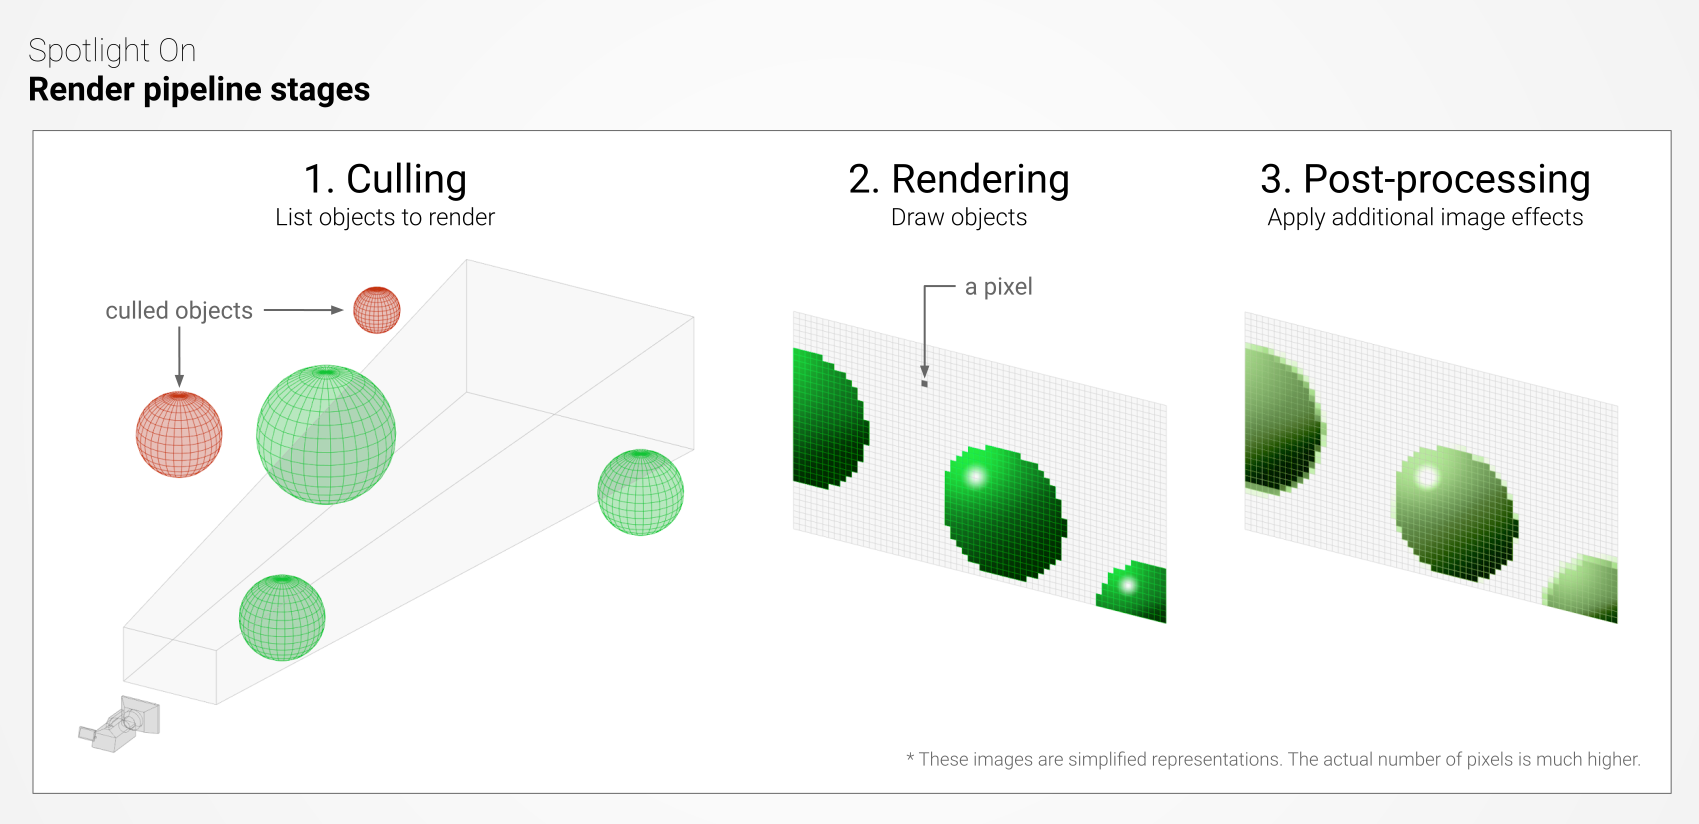
\includegraphics [scale=0.35] {my_folder/images//unity_pipeline}	
		\caption{Упрощенная схема конвейера отрисовки Unity} 
		\label{fig:unity_pipeline}  
	\end{figure}

	Предлагаемый конвейер сохраняет эту структуру, несмотря на изменения в алгоритме отрисовки, и требует 11 + S (где S - число источников света, отбрасывающих тень) вызовов отрисовки в \say{списке команд}, что видно по схеме конвейера на \firef{fig:pipeline_schema}. Каждый этап предствляет собой набор из подэтапов, где каждый подэтап решает ровно одну задачу.
	
	\begin{figure}[ht!] 
		\center
		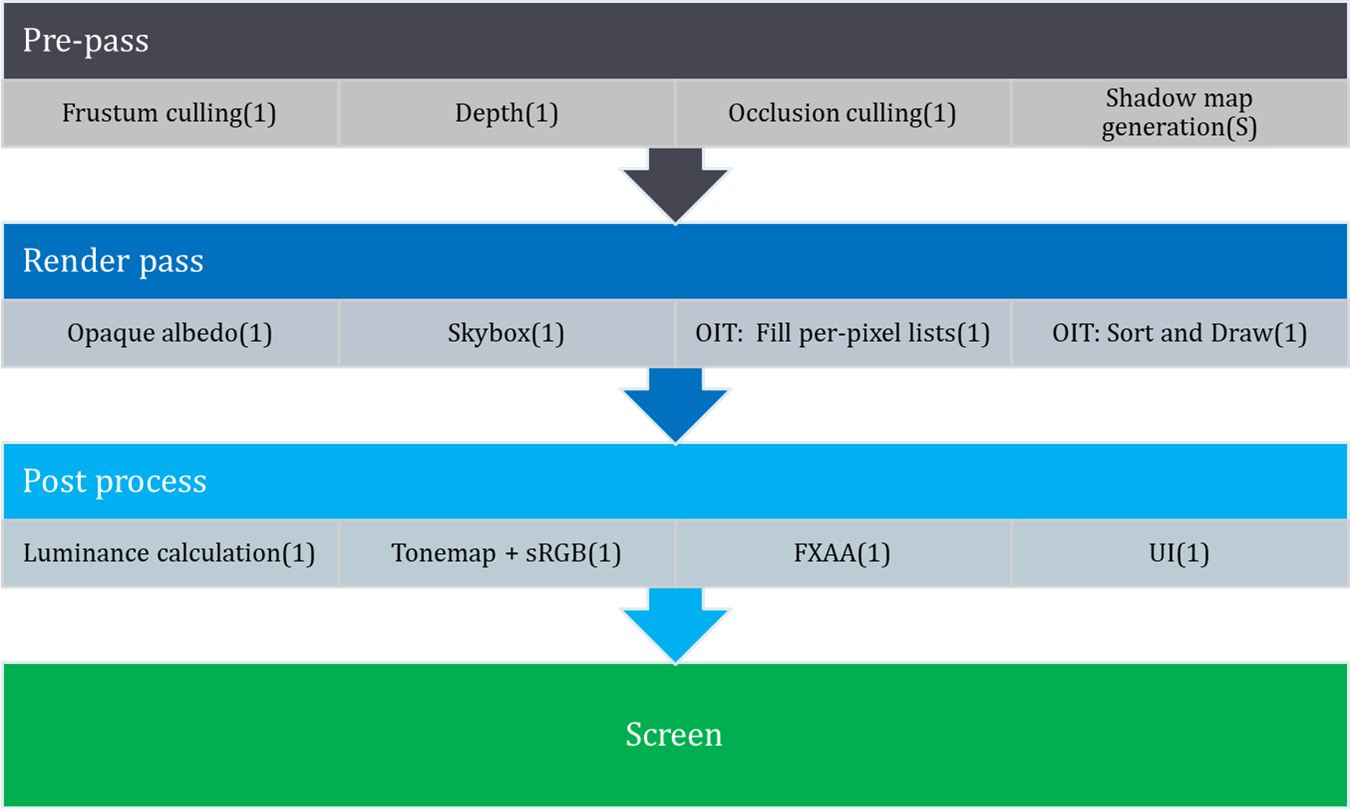
\includegraphics [scale=0.4] {my_folder/images//pipeline_schema}	
		\caption{Схема предлагаемого конвейера. В скобках указано количество вызывов ExecuteIndirect.} 
		\label{fig:pipeline_schema}  
	\end{figure}
	
	\FloatBarrier